\documentclass[11pt]{article}

% Packages for math and fonts
\usepackage{amsmath, amssymb, amsthm}
\usepackage[utf8]{inputenc} % Encoding
\usepackage[T1]{fontenc}    % Font encoding
\usepackage{geometry}       % Page margins
\usepackage{hyperref}
\usepackage{graphicx}

\geometry{margin=1in}
\setlength{\parindent}{0pt}    % No indentation at start of paragraphs
\setlength{\parskip}{1em}      % Vertical space between paragraphs


% Theorem environments
\newtheorem{theorem}{Theorem}[section]
\newtheorem{lemma}[theorem]{Lemma}
\newtheorem{definition}[theorem]{Definition}
\newtheorem{example}[theorem]{Example}
\newtheorem{remark}[theorem]{Remark}

\DeclareMathOperator{\R}{\mathbb{R}}
\DeclareMathOperator{\var}{var}
\DeclareMathOperator{\cov}{cov}
\DeclareMathOperator{\cor}{cor}
\DeclareMathOperator{\E}{E}
\DeclareMathOperator{\lgd}{\textit{lgd}}

% Title and author
\title{Expected Shortfall of a Bernoulli variable}
\author{Dominik Stich}
\date{\today}

\begin{document}

\maketitle

\section{Introduction}
We give a short note on the expected shortfall of a Bernoulli variable.

\section{ES of a Bernoulli variable}

Let \(L>0\) and \(X\in\{0, L\}\) a Bernoulli variable with \(P(X=L)=p=1-P(X=0)\).
We want to calculate the expected shortfall. To do this, we first need the distribution function \(F:\R\rightarrow\R\). Since this Bernoullivariable has atom mass in \(0\) and \(L\) and \(F\) is right continuous, we get
\begin{equation}
    F(x) = P(X\leq x) = \begin{cases}
        0 & \text{if } x < 0\\
        1-p & \text{if } 0\leq x < L\\
        1 & \text{if } L \leq x 
    \end{cases}
\end{equation}

The quantile function \(q:(0,1)\rightarrow [-\infty,\infty]\) is defined as \(q(u)= \inf\left\{x\in\R\vert F(x)\geq u\right\}\), which in this case yields

\begin{equation}
    q(u) = \begin{cases}
        0 & \text{if } 0 < u \leq 1-p\\
        L & \text{if } u > 1-p
    \end{cases}
\end{equation}

\begin{figure}[t]
  \centering
  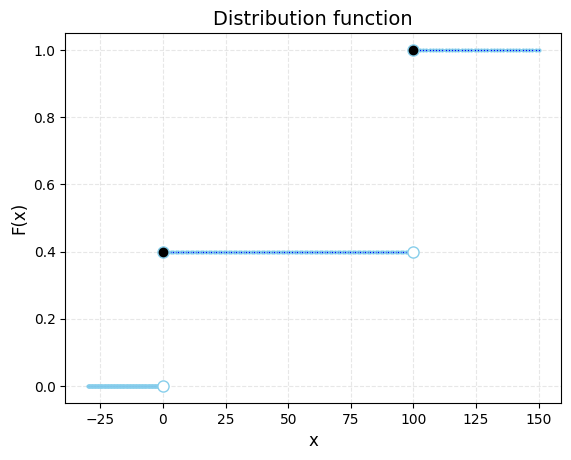
\includegraphics[width=0.4\textwidth]{F.png}
  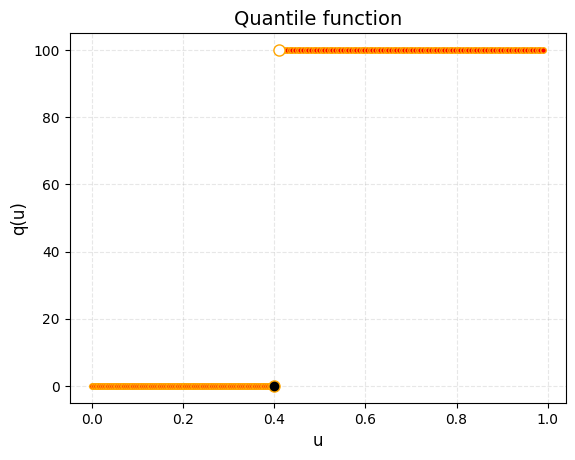
\includegraphics[width=0.4\textwidth]{q.png}
  \caption{The distribution and quantile function of a Bernoulli variable (\(L=100, p=0.6\))}\label{fig:quantile}
\end{figure}

Now let us compute the expected shortfall with level \(\alpha\in(0,1)\). By definition the expected shortfall of an \(\R\) valued random variable
at level \(\alpha\) is defined as

\begin{equation}
    \text{ES}_\alpha (X) = \frac{1}{1-\alpha}\int\limits_\alpha ^1 q(u)~du
\end{equation}

In the case of the above Bernoulli variable this yield:

\begin{align*}
    \text{ES}_\alpha (X) & = \frac{1}{1-\alpha}\int\limits_\alpha ^1 q(u)~du 
    \\&= \frac{1}{1-\alpha}\int\limits_{\max(1-p,\alpha)} ^1 L~du  
    \\ &= \frac{L * \left(1-\max(1-p,\alpha)\right)}{1-\alpha} 
    \\&= L \min\left(\frac{p}{1-\alpha},1\right) 
\end{align*}

\textbf{Interpretation:} 
To interpret this result, it is easiest to look at the alternative formula for expected shortfall:
\begin{equation}
    \text{ES}_\alpha (X) = \frac{1}{1-\alpha}\left(\text{E}\left[X 1_{\{X> q(\alpha)\}}\right] + q(\alpha)\left[P(X\leq q(\alpha))-\alpha\right]\right)
\end{equation}
which holds for general distribution functions.

For \(\alpha<1-p\), we have \(q(\alpha)=0\) and the formula reduces to
\begin{equation*}
    \text{ES}_\alpha (X) = \frac{1}{1-\alpha}\text{E}\left[X 1_{\{X> q(\alpha)\}}\right]=\frac{p}{1-\alpha}=\frac{EX}{1-\alpha}
\end{equation*}

This means, when we simulate \(N\) Bernoulli, we just count the default events \(\approx Np\) and divide by \(1-\alpha\), 
which will be smaller than \(1\), meaning that there are non default events contributing to the tail.

If on the other hand \(\alpha \geq 1-p\), then \(q(\alpha)=L\), so \(\{X>L\}=\emptyset\), \(P(X\leq q(\alpha))=1\) and the formula becomes

\begin{equation*}
    \text{ES}_\alpha (X) = \frac{1}{1-\alpha}L\left[1-\alpha\right]=L
\end{equation*}

every single event contributing to the expected shortfall is a default.

\end{document}
